\documentclass{sigchi}

\def\nimi{Supporting Exploratory Search with User Modeling}
\def\tuire{Tuire Peurala}
\def\ilkka{Ilkka Kiistala}
% Use this command to override the default ACM copyright statement (e.g. for preprints). 
% Consult the conference website for the camera-ready copyright statement.
\toappear{
Submitted for review.
}

% Arabic page numbers for submission. 
% Remove this line to eliminate page numbers for the camera ready copy
\pagenumbering{arabic}
% Load basic packages
\usepackage{balance}  % to better equalize the last page
%\usepackage{graphics} % for EPS, load graphicx instead
\usepackage{graphicx}
\usepackage{times}    % comment if you want LaTeX's default font
\usepackage{url}      % llt: nicely formatted URLs

\usepackage{csquotes}

% llt: Define a global style for URLs, rather that the default one
\makeatletter
\def\url@leostyle{%
  \@ifundefined{selectfont}{\def\UrlFont{\sf}}{\def\UrlFont{\small\bf\ttfamily}}}
\makeatother
\urlstyle{leo}


% To make various LaTeX processors do the right thing with page size.
\def\pprw{8.5in}
\def\pprh{11in}
\special{papersize=\pprw,\pprh}
\setlength{\paperwidth}{\pprw}
\setlength{\paperheight}{\pprh}
\setlength{\pdfpagewidth}{\pprw}
\setlength{\pdfpageheight}{\pprh}

% Make sure hyperref comes last of your loaded packages, 
% to give it a fighting chance of not being over-written, 
% since its job is to redefine many LaTeX commands.
\usepackage[pdftex]{hyperref}
\hypersetup{
pdftitle={\nimi},
pdfauthor={\ilkka  and \tuire},
pdfkeywords={Seminar paper, Literature review, Exploratory search},
bookmarksnumbered,
pdfstartview={FitH},
colorlinks,
citecolor=black,
filecolor=black,
linkcolor=black,
urlcolor=black,
breaklinks=true,
}

\DeclareGraphicsExtensions{.pdf,.png,.jpg}

% create a shortcut to typeset table headings
\newcommand\tabhead[1]{\small\textbf{#1}}


% End of preamble. Here it comes the document.
\begin{document}

\title{\nimi}

\def\tktl{Department of Computer Science\\University of Helsinki}
\def\tktladdr{P.O. Box 68 (Gustaf H\"allstr\"omin katu 2b)\\
FI-00014 UNIVERSITY OF HELSINKI\\
FINLAND}

\numberofauthors{2}
\author{
  \alignauthor \ilkka\\
    \affaddr{\tktl}\\
    % \affaddr{\tktladdr}\\
    \email{ilkka.kiistala@helsinki.fi}
  \alignauthor \tuire\\
    \affaddr{\tktl}\\
    % \affaddr{\tktladdr}\\
    \email{tuire.peurala@helsinki.fi}
}

\maketitle

% include abstract.tex as commands
\begin{abstract}
In this literature review we introduce exploratory search and cover three techniques that help users in succeeding in their exploratory search tasks efficiently. Exploratory search is an information retrieval strategy that combines learning and investigation activities. We explain the concept of exploratory search and what distinguishes it from other information retrieval strategies. Exploratory searchers can be supported in their tasks by means of user modeling. After shortly summarizing user modeling we present three practical techniques that combine user modeling with exploratory search. 
\textit{Faceted search} is a method where structured metadata is used to provide the user with an overview of the results and clickable categories. 
\textit{Relevance feedback} provides the user an option to rate the usefulness of the result. This information is used in ranking the search results next time. 
\textit{Query term suggestion} displays choosable query suggestions as the user is typing their query.
\end{abstract}


\keywords{
Exploratory Search; 
Information Retrieval;
User Modeling.
Faceted Search;
Relevance Feedback;
Query Term Suggestion;
}

\category{H.5.5.}{Information Interfaces and Presentation (e.g. HCI)}{Modeling}

\section{Introduction}
Modern day people live in an information-rich world. Information is available to people at any time at any place and in any form and this may lead to information overload. The information needs vary by the task-at-hand, the user and the context. There is a growing need to somehow prefilter and narrow down the knowledge domain to make it possible to succeed in demanding and ambiguous information-seeking tasks. Information retrieval tasks the users execute are different, and it has been shown that there are different categories of searching \cite{kuhlt91}. In this literature review we introduce exploratory search and how a system can help users to fulfill their needs. We adopt the description of exploratory search by Marchionini: 

\blockquote{Exploratory search can be used to describe an information-seeking problem context that is open-ended, persistent, and multi-faceted; 
and to describe information-seeking processes that are opportunistic, iterative, and multi-tactical. 
In the first sense, exploratory search is commonly used in scientific discovery, learning, and decision-making contexts. 
In the second sense, exploratory tactics are used in all manner of information seeking and reflect seeker preferences and experience as much as the goal \cite{march06}.}

An exploratory search task differs notably from a search task with a well-defined objective.
In the latter the user stops after finding an answer to a question.
The goal is reached as the need of information is fulfilled.
The exploratory searchers are possibly exploring a domain where they have a general interest but no specific knowledge.
As the searcher is not after a specific fact, the search process is iterative, accumulating insight, and the user might return to the task several times and possibly in several sessions making the task persistent.
It is characteristic for exploratory search to include stages where user redefines the goal and may find new direction in their search task as their understanding grows.
The means of exploring may include multiple applications and information sources.
The nature of an exploratory search is that the information need is broad.
Supporting this sort of constantly evolving and opportunistic approach is challenging, because the tactics and preferences vary.
Although the evaluation of exploratory search user interfaces has been proven to be difficult \cite{white09}, some design guidelines have been proposed and some solutions have been found to help users in their exploratory search tasks.
To this literature review we chose three solutions that are seen in search systems in general, but these solutions can be enhanced further by utilizing user modeling.

To build a good system where computer and human cooperate to perform a task it is important to take into account some significant characteristics of the user \cite{rich99}.
User model is built of these characteristics.
User models are used in adapting the system for the users.
Fischer defines user models as follows:

\blockquote{User models are models that systems have of users that reside inside a computational environment \cite{fischer01}. }

Traditionally a user model has been a model of a typical user \cite{rich99}.
In reality, often the users vary so much that a traditional user model is insufficient and there is a need for a more specific user model describing an individual user.
A central objective of user modeling is to address the problem that system will be unable to interact with users cooperatively unless it has some means of finding out what the user really knows and does \cite{fischer01}.
Since the user's goals may change during the use of system there is a need to refine the user model during the course of the task.
User information for building a model may be gathered explicitly from the user by asking questions or implicitly by recording and analyzing user's interactions with the system.
Implicit sources of user information are for example looking at the commands or patterns of commands the user uses.
When the user model is complex the time to gather facts to fill up the needed information one by one takes too much time.
In this situation a sterotype can be used to infer many things at a time.
Human traits often occur in clusters and if it is known that a user likes Battlestar Galactica it may be inferred that he is also interested in other science fiction series. 

In order to accommodate to differing needs of users or user groups over time, a system may use one of three basic approaches \cite{van08}: System is called \textit{adaptive} if it alters its structure, functionality or interface on the basis of a user model generated from implicit user input; in \textit{Adaptable} systems the user model is constructed with explicit user input and so it requires user's active participation; \textit{Personalized} system is a hybrid of the two aforementioned. 

In this literature review we introduce the problem of exploratory search and some solutions for the problem.
We explain what exploratory search is and what distinguishes it from other information retrieval tasks.
We cover three techniques that help the users to succeed in their exploratory search tasks efficiently.
The chosen solutions were selected, because 1) they are already widely used in practise, 2) they take place in different stages of the search process and 3) their use of user modeling differs.
We describe how exploratory search process benefits from the use of user modeling in these three solutions.

In the following chapter we introduce basic concepts of exploratory search and user modeling.
After that we present some solutions and systems supporting exploratory search that we found exploring the literature.
In the Discussion chapter we summarize our findings and present our newly-found insight and the concerns that emerged while exploring the topic.

\section{Literature review}
\label{sec:litreview}

% include as commands
\subsection{Exploratory Search}
The search for information and extending one's knowledge is a built-in behaviour in humans.
Last few decades have transformed search and made it an everyday function.
It wasn't until the late 1990's until web search services began offering quick access to information and changed the ways of information seeking.
Before the Web, information search services were used mainly by academics and information professionals.
With a small amount of users, the search system manufacturers didn't need to focus on the user experience and had no motivation to improve the user interface.
Traditional search systems were lookup-based and as such, the query formulation was an essential stage of the search task.
Some studies mention systems, where the query results took days to return . In such cases, the (user learns the system very slowly), since becoming a better user of such a system requires interaction with system and slow (query return) means slow learning.

Search system must be quick for other reasons too. Cognitive abilities restrict the searcher from running other tasks and starting sub-tasks in parallel with the original task []. That means the system should be simple and support user's (state of mind), not adding to the cognitive load already affecting the user. Whenever the user needs to (think on a higher level) it's possible the ‘flow' of the search task is lost. This so-called flow is a state of mind that the searcher has and having to set that aside might result in losing it.

The flow however, is not so important when the search task is simple. Let's think of a simple search task: a teacher has assigned a group of students to draw a poster about a European country and the group have chosen Denmark. They want to display some facts about the country in their poster, for example the population, land area and internet top-level domain. To retrieve these facts, a simple search with keyword Denmark will suffice.
The facts can be copied from Wikipedia or the official website of Denmark to the poster.
This kind of lookup-based information retrieval model is described in Figure \ref{figure_classicIR}.

\begin{figure}[htp] % t=top, h=here, b=bottom, p=separate page, !=place even if ugly
\caption{The classic information retrieval model. Based on \protect\cite{bates89}.}
\label{figure_classicIR}
\centering
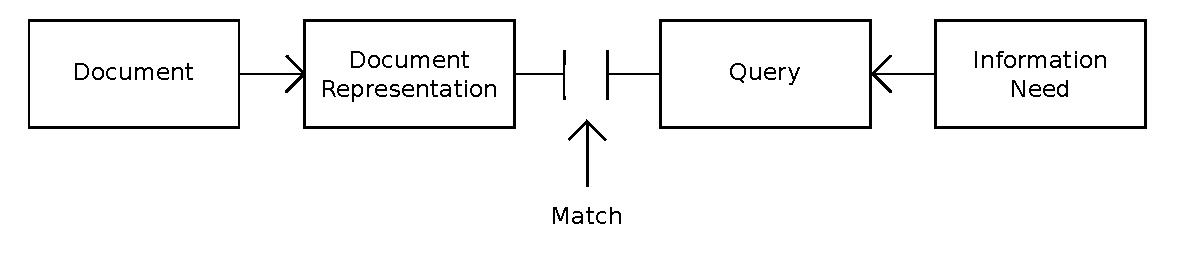
\includegraphics[scale=0.45]{figures/classicIR.pdf}
\end{figure}

After finishing the poster, the group is given a new assignment.
Their second assignment is to write a short play of any historical event that was of special importance for Denmark and then perform the play in front of the class.
This time, the information needed for completing the assignment can not be clearly defined. 
Compared to the previous assignment, it takes much more time.
Estimating the needed time and effort is harder, because the goal is not as clear as it was with the previous assignment.

The students might start by reading the history of Denmark in the Wikipedia.
Along their exporation, they come upon different events and characters that have had an effect in Denmark's history and make new queries regarding the newly-found topics.
The information seeking process described here fits well in what is said of berrypicking behaviour (See Figure \ref{figure_bp}).
In berrypicking behaviour the searcher gets new ideas and new paths to follow as they browse the search results of their search query. In the example, as the students are reading about the 10th century events in Denmark, they might get interested in Harald Bluetooth, the King of Denmark at the time, and begin searching for information of him.  

\begin{figure}[htp] % t=top, h=here, b=bottom, p=separate page, !=place even if ugly
\caption{An evolving berrypicking search. Based on \protect\cite{bates89}. From \protect\cite{march06}.}
\label{figure_bp}
\centering
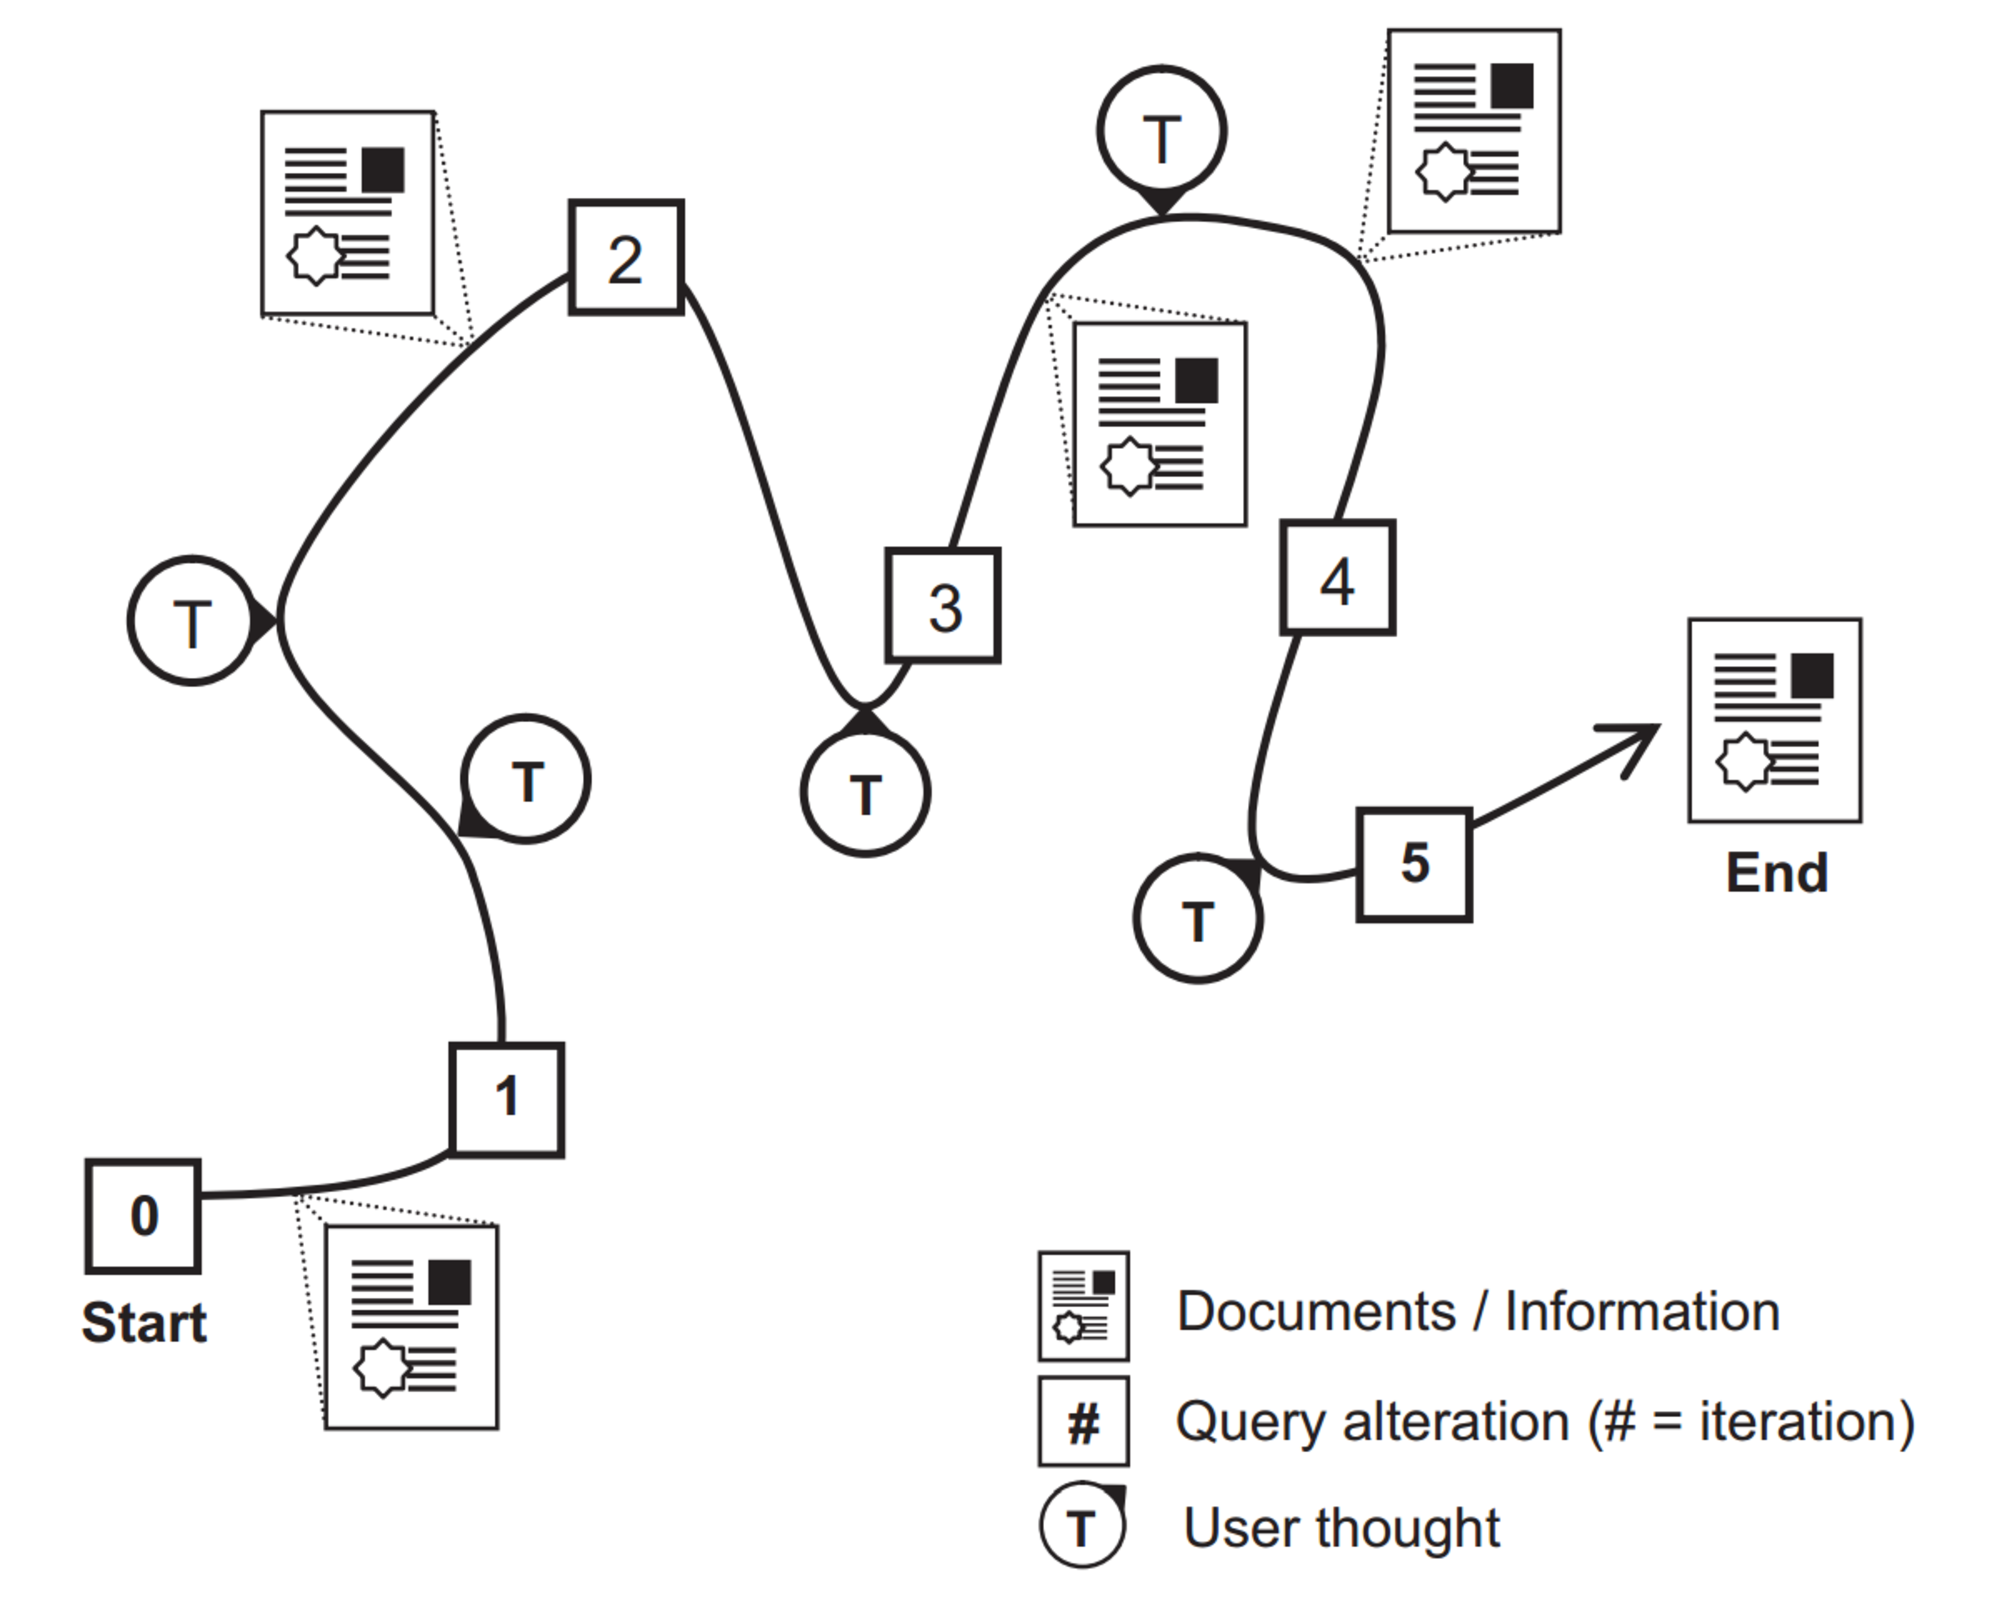
\includegraphics[scale=0.25]{figures/berrypicking.pdf}
\end{figure}

Bates \cite{bates89} describes the berrypicking approach as "evolving search", because during the process the desired outcome may change, as well as the query.

With their now improved knowledge of Danish history, they need to decide which event to depict in their play.
This requires collaboration within the group, which is typical for exploratory search activities.
After decision on the event, the group needs to gather information to be able to write a script for the play.
They have to do some research on the people involved in the selected historical event and if necessary, they must seek for information on what kind of clothes were used in the era the event took place in.
The previously used websites might lack the information they are after so the searchers have to find new sources of information and their search strategies may change.
As seen in Figure \ref{figure_bp}, new information results in query alterations or user thoughts.
Bates \cite{bates90} described a four-level hierarchy of search activities within berrypicking: move, tactic, stratagem and strategy.
Single physical or mental actions by the user are moves, and tactics are a combination of moves. 
Berrypicking could be described as complex combination of moves and tactics, whereas lookup-based information retrieval is a simple set of tactics and moves \cite{white09}.

\begin{figure}[htp] % t=top, h=here, b=bottom, p=separate page, !=place even if ugly
\caption{Different search tasks are split into three overlapping search activities: \textit{lookup}, \textit{learn} and \textit{investigate}. Based on \protect\cite{march06}.}
\label{figure_3clouds}
\centering
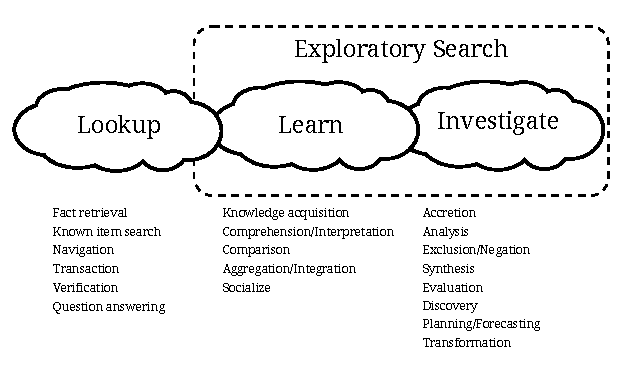
\includegraphics[scale=0.8]{figures/3clouds2.pdf}
\end{figure}

Introduction to exploratory search. See Figure \ref{figure_3clouds}.
\cite{march06}, \cite{white09}, \cite{tvaro11}

The user interface of an exploratory search system should be designed to fulfill the needs of most of its users. More information on what works and doesn't work can usually be collected from system evaluations.
However, evaluating exploratory search systems is difficult, because users have different starting positions. Their knowledge of the domain varies, they are interested in different aspects of the topic and they have previously encountered different information. \cite{kules08}

Exploratory search and iterative search differ. See Figure \ref{figure_IterativeVsExploratory}.

\begin{figure}[htp] % t=top, h=here, b=bottom, p=separate page, !=place even if ugly
\caption{They differ. From \protect\cite{white09}.}
\label{figure_IterativeVsExploratory}
\centering
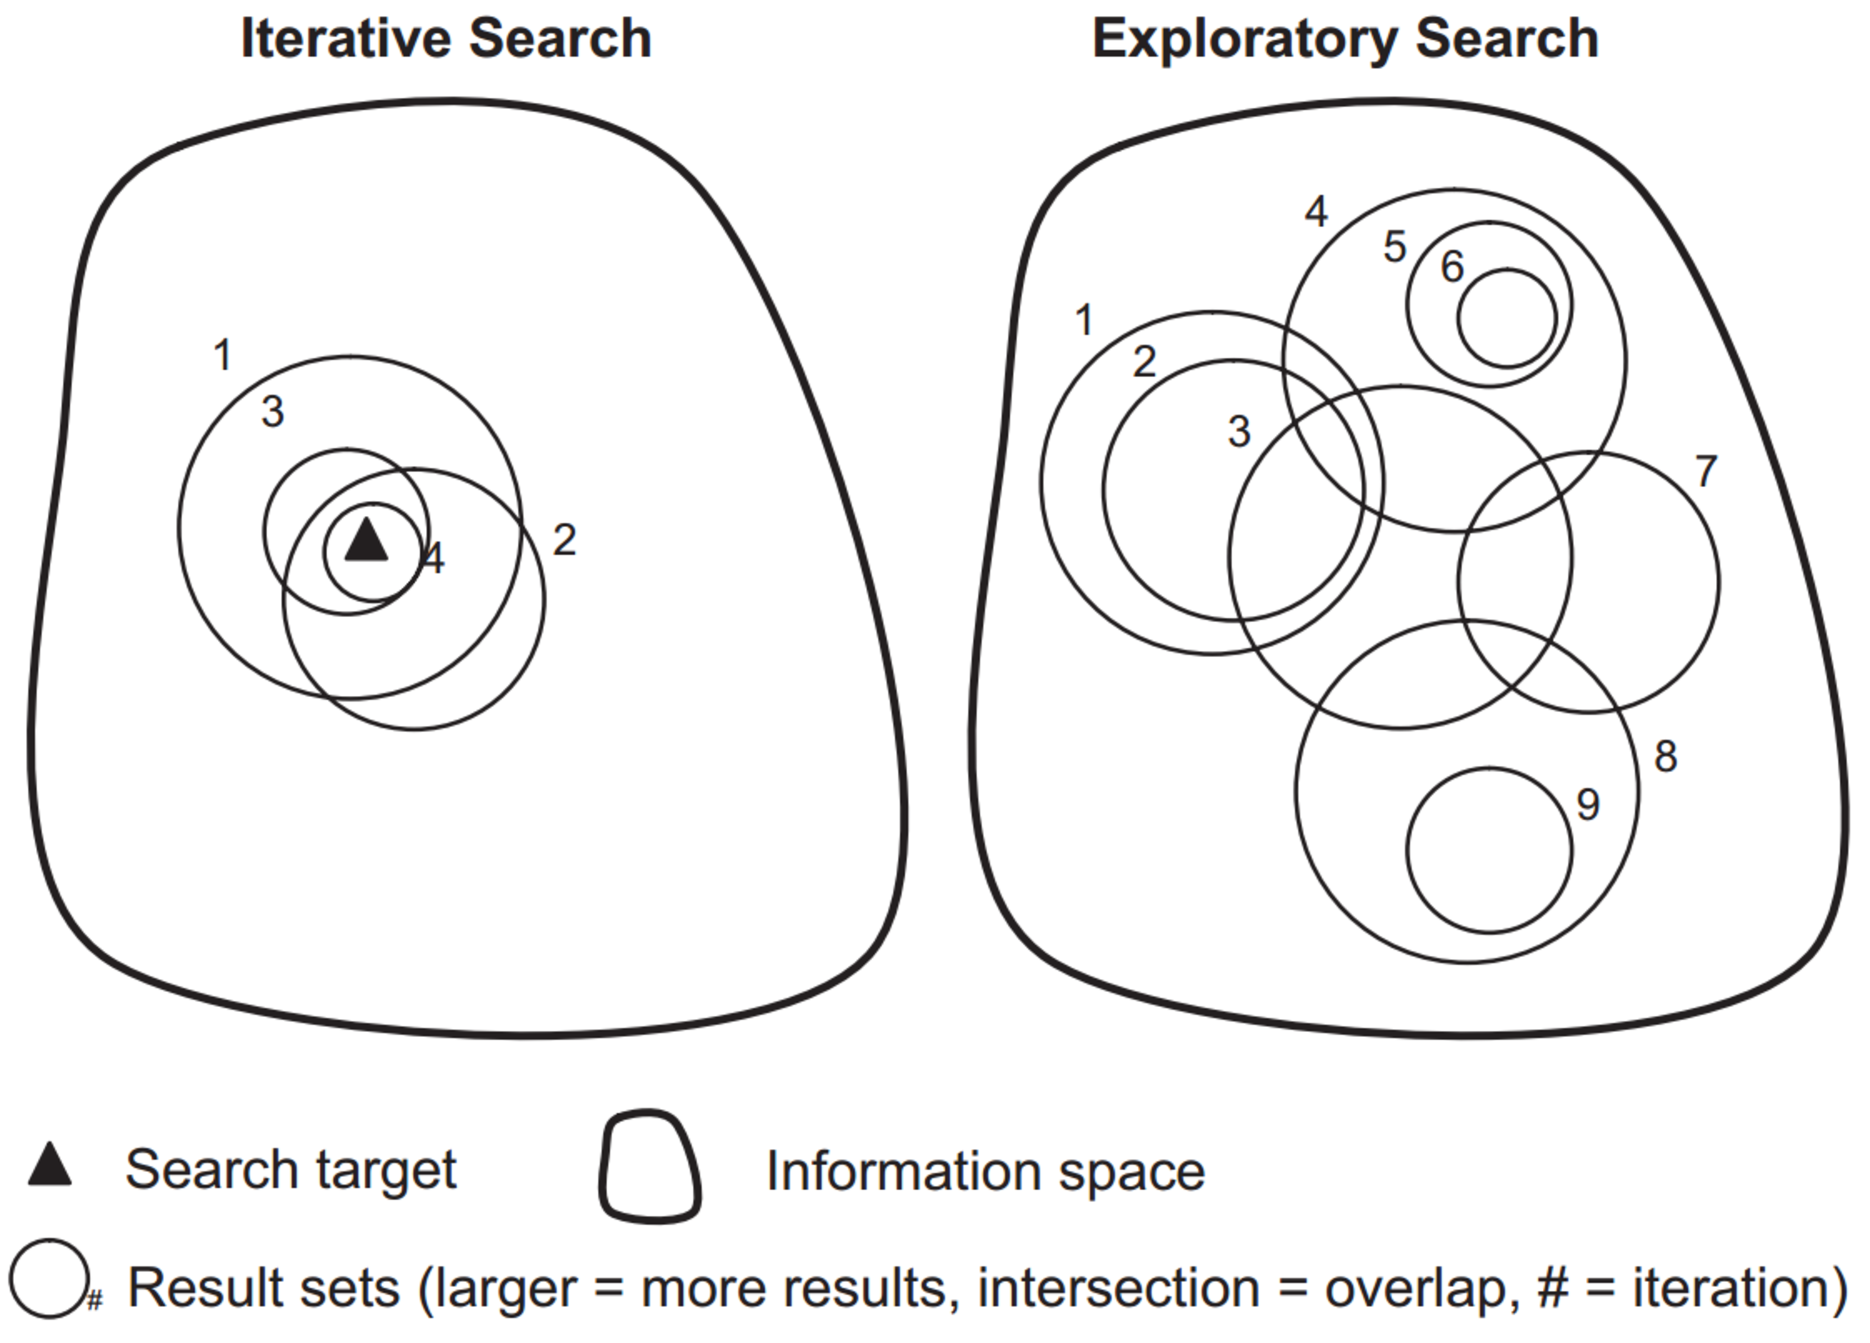
\includegraphics[scale=0.25]{figures/IterativeSearch_vs_ExploratorySearch.pdf}
\end{figure}

Exploratory search tasks can be characterized as either learning oriented or investigative  and they have common aspects like uncertainty, ambiguity and discovery distinguishing them from look-up oriented tasks \cite{kules09}.



\subsection{User Modeling}

In the first ten years of Human-Computer interaction history the focus of research was in user interfaces and particularly the possibilities and design criteria of graphical user interfaces \cite{fischer01}. Later the focus has moved toward more broadly improving the way people use computers for example to work, think, communicate and learn \cite{fischer01}. To build a good system where computer and a human cooperate to perform a task it is important to take into account some significant characteristics of people \cite{rich99}. User models are built of these characteristics and are used to adapt the system toward the user.

A central objective of user modeling is to address the problem that system will be unable to interact with users cooperatively unless they have some means of finding out what the user really knows and does \cite{fischer01}. To find out this there are two communication channels the explicit user input and the implicit information that is gathered without any effort from the users. The data gathered through these channels is combined to the background knowledge of the problem domain, communication processes and the user agents involved and is then used to improve the interaction with the system (see Figure \ref{know_hci}).

\begin{figure}[htp] % t=top, h=here, b=bottom, p=separate page, !=place even if ugly
\caption{Knowledge-based HCI \protect\cite{fischer01}.}   \label{know_hci}
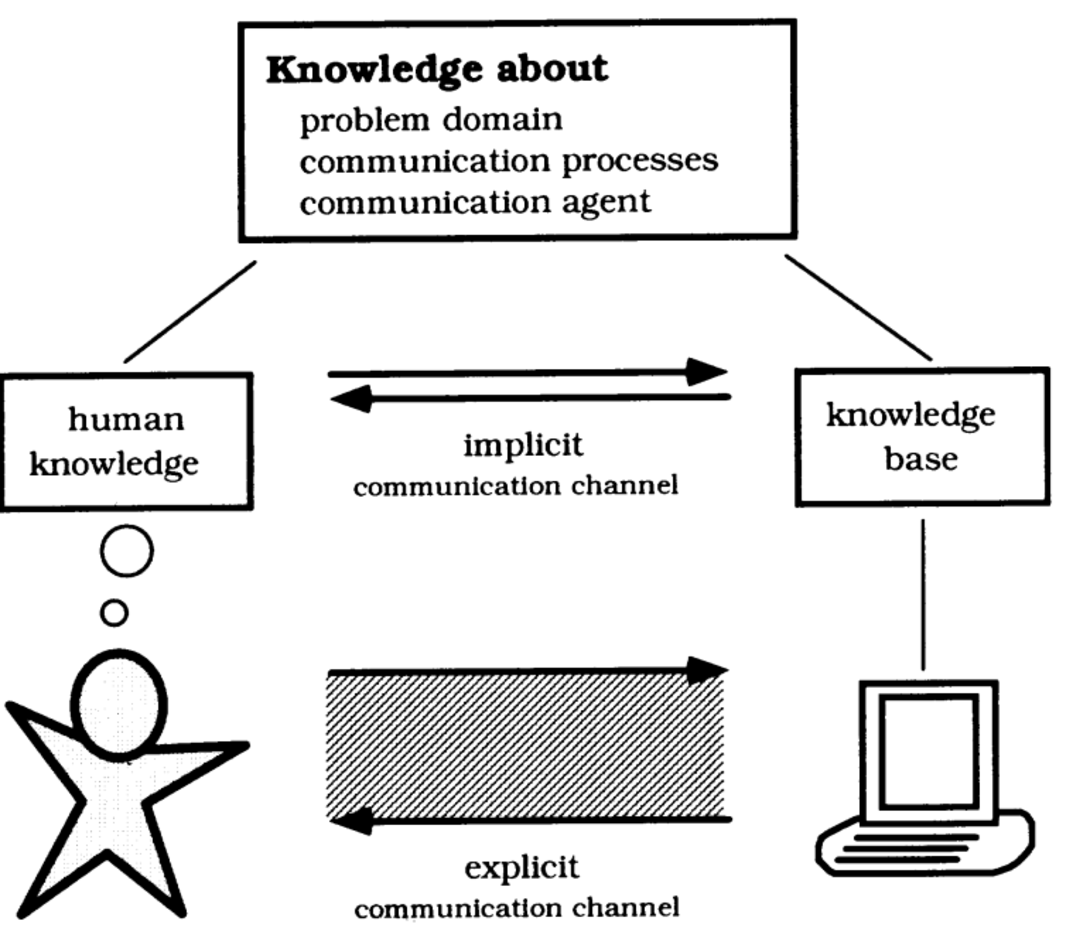
\includegraphics[scale=0.45]{figures/knowledge_hci.pdf} 
\end{figure}

In order to accomodate to differing needs of users or usergroups over time, a system may use one of three basic approaches \cite{van08}. System is called \textit{adaptive} if it alters it structure, functionality or interface on the basis of a user model generated from \textit{implicit} user input. \textit{Adaptable} systems use \textit{explicit} user input and need user's active participation. \textit{Personalized system} is a hybrid of the two aforementioned. In personalized systems the output or appearance differs for every user or user group in every context \cite{van08}. The adapted output has the potential to be of great benefit for users; it is geared towards the user's preferences, behaviour and needs and it can make interaction easier and a lot more fruitful. Including adaptive elements in the user interface might increase the workload of the user. When users had two alternative interfaces to a menu, an adapted one and a full one, there was cognitive overhead in 1) having to decide which features to include in the personalized interface and 2) having to figure out a menu item was missing and that changing to the full interface would make it appear in the menu again \cite{bunt04}. In general the lifecycle of a computational system cannot anymore be divided to the design time and use time as the behaviour of system can adapt to contextual information like the user goals only known at the use time. The differentiation between the design time and the use time of the system gets blurred with user modeling and the use time becomes also design time \cite{fischer01}.

The different types of user models can be mapped as a three dimensional space where the axes are: single model vs. collection of models, explicitly specified models vs. models inferred by the system on the basis of user behaviour and long-term vs. short-term user models \cite{rich99}. The user model classification map is depicted in Figure \ref{dim_UM} and the three dichotomies are explained further in this chapter. 

\begin{figure}[htp] % t=top, h=here, b=bottom, p=separate page, !=place even if ugly
\caption{The dimensions of user modeling.} \label{dim_UM}
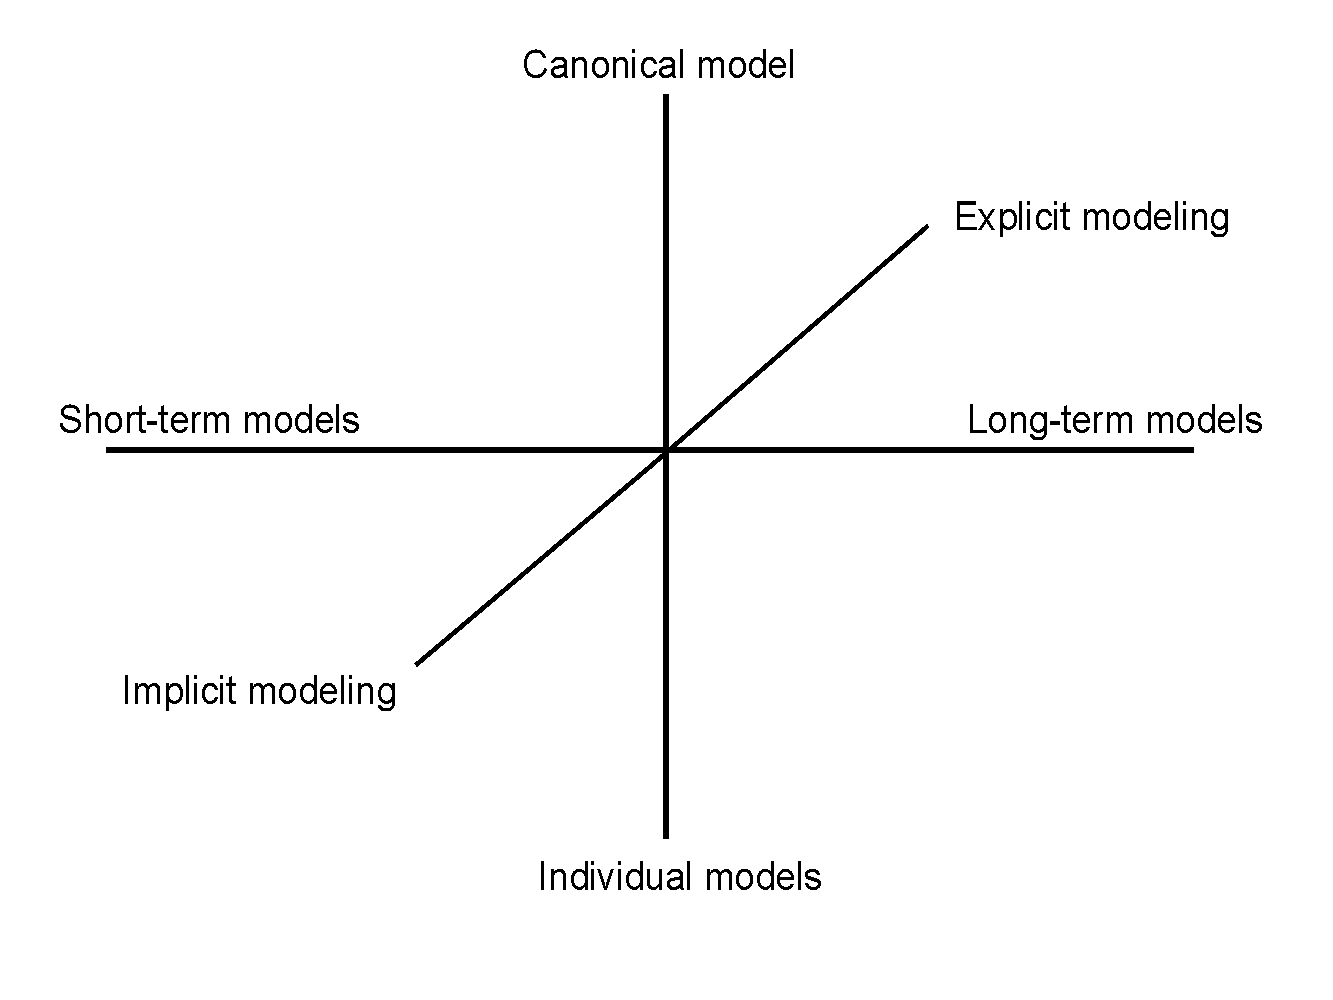
\includegraphics[scale=0.4]{figures/dimensions_UM.pdf} 
\end{figure}

The \textit{single model vs. collection of models} polarity \cite{rich99} has on it's other end the single model of single user. The modeled single user is called the canonical user and is actually not a real person at all but a modeled stereotypical user of the system. Traditional user models have been constructed by collecting data on an average user on various tasks and environments \cite{rich99}. An example of a canonical user model is Fitt's law that suggests that the speed on which the user operates the machine can be increased by increasing the size of targets the user must hit. The major weakness of these kind of models is that they assume that all the users constitute a homogenous set. In most cases for the majority of users the system is better adapted to them that would be without any adaptation, but it isn't likely the best system that could be produced \cite{rich99}. In the other end of this dichotomy is the collection of models of individual users. These users are real and the facts to build the individual model are gathered usually from the interaction of the user with the system. When choosing whether to use a canonical or individual user models one should think if the canonical model is sufficient or is the user community too heterogenous for it to be useful enough \cite{rich99}. The decision on this axis influences the other aspects of user modeling. If one user model is used then it has to be designed only once and the system doesn't have to prepare for incorrect or conflicting user model information as the case is on the latter option. 

The way how the user model is specified forms the second dichotomy mapping the user modeling techniques; \textit{explicit vs. implicit models} \cite{rich99}. On the explicit side the model is specified explicitly either by the system designer or by the users themselves. User model may be formed by letting the user modify the system but this leaves a lot on the hand of the user and fits badly to systems that expect to have lot of users that use the system only once or twice. Explicit user modeling can be done also by asking questions directly from the users but one problem with this is that users can't always answer on what the system needs to know. On the other end of the axis models are formed more subtly, they are inferred by the system only on the basis of user's behaviour. Implicit user models are built by gathering information of the user when the user interacts with the system. When constructing the user model implicitly the system must have some way of distinguishing incorrect information and resolving conflicts between gathered information.

In order to adapt soundly to the user the system must have wide variety of information about the user. The information might be ranging from short-term facts like the last query the user performed to more long-term facts like the level of mathematical sophistication of the user. This forms the third dichotomy: \textit{long-term vs, short term user models} \cite{rich99}. Long-term models can be built in the course of series of interactions between the system and the user. Long-term model could be built for example in a bookstore application where information of the user's purchases might be gathered to to recommend books of certain genre for the user. Short-term user model could be used in a search application. The model would be built by gathering recent queries to form a model of the user's search goal. Short-term user model is needed to respond to a situation where a user would need different search results when searching with keyword “Java” after searching information on programming or after the user has been searching beaches in Indonesia. There are also other differences in user models besides these introduced three dichotomies. Example of these differences is the model lifecycle; in a system where there is only a single model it can be permanently embedded with the system but in the case where there are models for each individual user the model is built on the fly. This and many other differences follow from the aforementioned three axes and are not distinguished as categorizing user models \cite{rich99}. 

User model building techniques are many. System may try to identify the user's vocalbulary and interpretation of concepts \cite{rich99}. In another technique the results that user seems to be satisfied with are assessed to gather facts for the model \cite{rich99}. Still another technique is to use stereotypes to generate many facts from a few \cite{rich99}. Generally user model building techniques may be divided into two clusters; the ones inferring \textit{individual facts} and the other ones using \textit{stereotypes} to infer many things at a time \cite{rich99}. Individual facts may be gathered at its simplest by looking at how the users use the system. An expert will use more advanced commands than a beginner. The patterns of commands may be interpreted to know whether the response given by the system was satisfactory. If the user tries to find information from the system and after the response leaves or continues to other search it may be assumed that he found what he was looking for. Instead, if the user restructures his query it may be assumed the result was not sufficient. This feedback may be used in building a user model. If a user model is very complex it may be too time-consuming to try to fill it by gathering facts one by one, then it is possible to try to infer many facts by using stereotypes. Human traits are not scattered randomly throughout the population instead they occur in clusters of traits. A single trait may imply a whole cluster of traits like a person that is interested in organic food may also be interested in recycling and public transport.  The clustering of facts may also be broadened to events. It is common that events neiher do occur in random order but they as well have patterns of occurance that can be used in user modeling. For example in shops people gather items they need, go to the cashier, pay their purchases, wrap them up and leave the shop. The concept of stereotype has many negative assosiations but the technique still is usable in capturing the structure in the context of user modeling. Still it must be taken into account that a stereotype only states that sometimes some traits occur together not that they always do and so a triggering trait may be seen only suggesting existance of a particular stereotype. 

It has been suggested that using single user model of canonical user in interactive systems is not enough to satisfy the heteregenous user community \cite{rich99}. Rather, there is a need to build user models of individuals to make human-computer interaction more efficient and collaborative in nature. 
The shift to the direction of personalization leads to challenges in building user models but also on the other hand evaluation of systems becomes more demanding. The evaluation of a personalized system is problematic because it is unclear if the results gathered from a few individuals who all have used the system personalized for them can be generalized to entire population of users \cite{van08}.

Search systems have evolved from simple "query to results" paradigm to a clever systems that utilize the user models to provide the user with better search results. Instead of providing results based on solely the search word, the search system can extend the search beyond the search terms and, for example, include some synonyms in the query. Or the search system might recognize a common typo in the search query and replace the misspelled word with the correct one. The system might ask the user to rate the result of the search and then change accordingly. In the following subsections we cover three different solutions that support exploratory search and may be further enhanced with user modeling. The solutions are faceted search, relevance feedback and query expansion.
PUUTTUU:\cite{bunt04}, \cite{findlater04}, \cite{brusi96}

\subsection{Faceted search}

Information seekers often express a desire for a user interface that organizes search results into meaningful groups, in order to help make sense of the results and to help decide what to do next \cite{hearst06}. Exploratory search is a complex information seeking task and to support this it has become accepted to use faceted search or categorized overviews \cite{kules09}. In faceted search structured metadata is used to provide the user with an overview of the results and clickable categories. There are two ways of grouping search results; clustering and hierarchical faceted categories. Clustering is grouping of items based on some similarity and is fully automated process. It is good for clarifying a vague query but the clustering algorithms aren't yet perfect and the clustering can be unpredicted \cite{hearst06}. Category system is a set of labels that are organized to mirror the domain. Hierarchical faceted categories are a set of hierarchical categories that each represent a different dimension. Categories are usually created manually but can be partly automated. Traditional categories place a document inside single category but facets allow document to exist simultaneously in multiple overlapping taxonomies \cite{koren08}. Faceted interfaces have three characteristics; they present a number of facets and facet values, query can be interactively refined via the facets and users can remove previously selected facets \cite{koren08}. 

\begin{figure*}[ht!] % t=top, h=here, b=bottom, p=separate page, !=place even if ugly
\caption{ Faceted Search: Flamenco system} \label{flamenco}
\centering
\vspace{5pt}
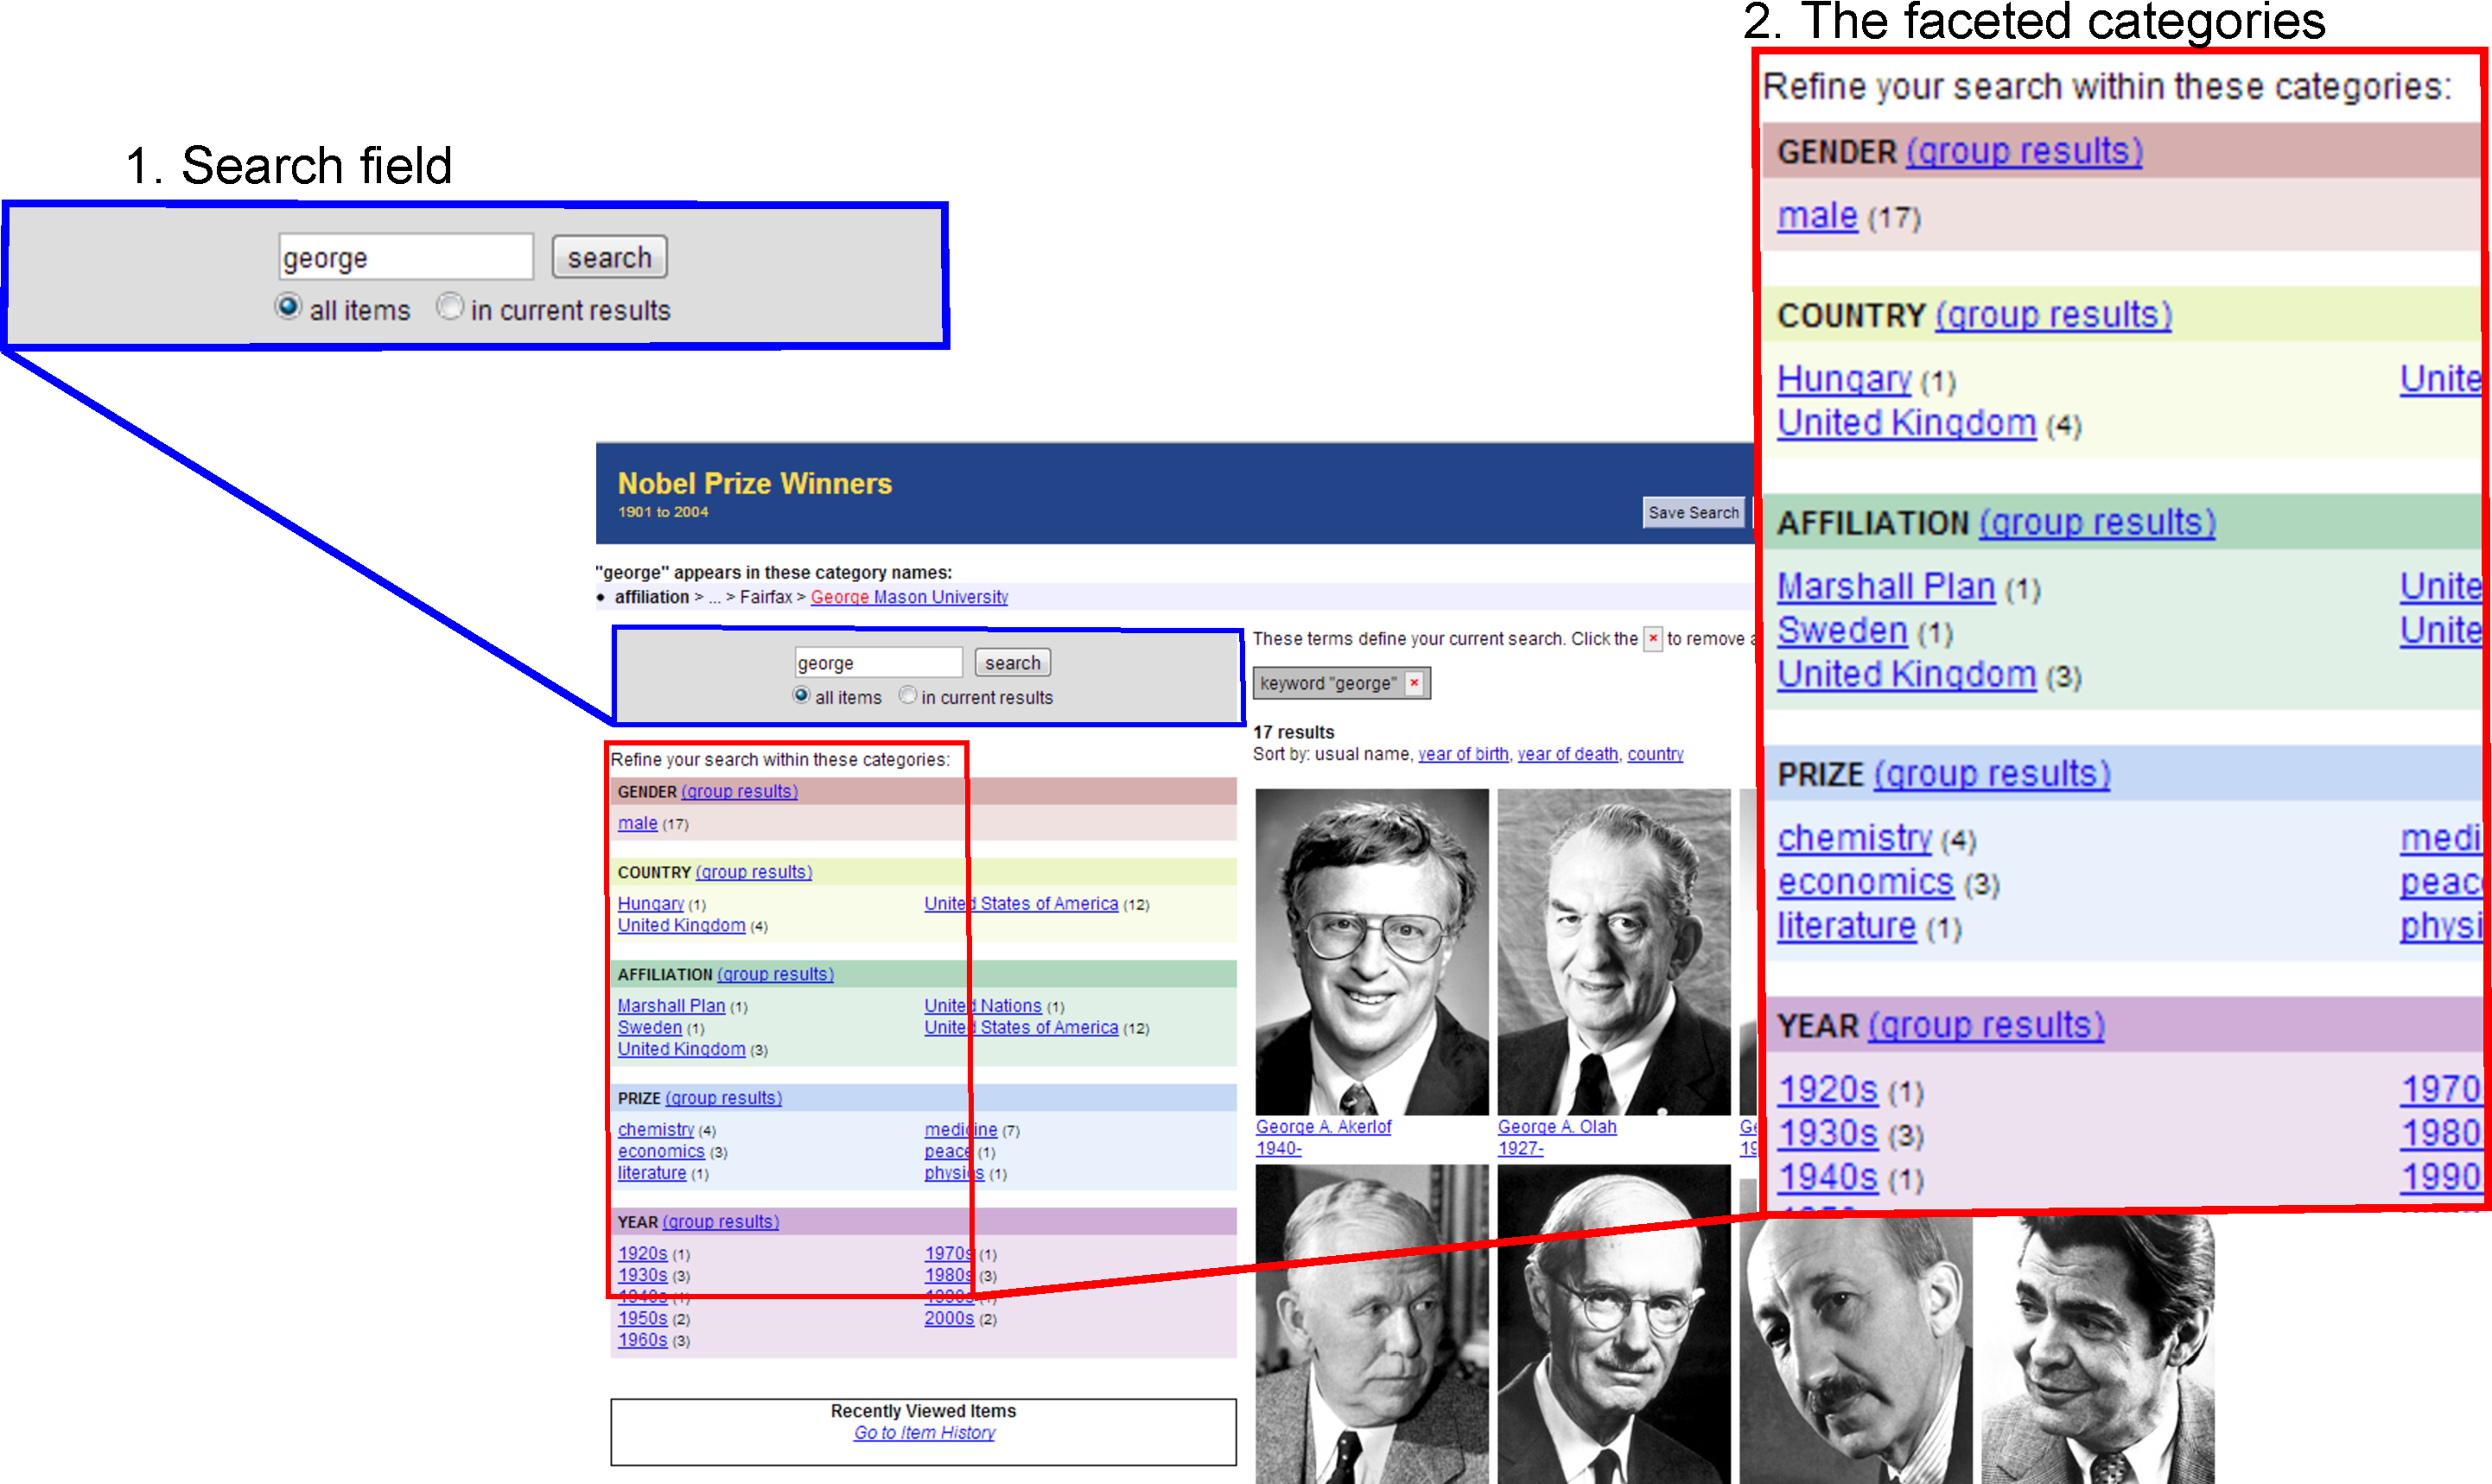
\includegraphics[scale=0.28]{figures/flamenco.pdf} 
\end{figure*}

An example of faceted search interface can be seen on Figure \ref{flamenco}. The user interface in the figure is an experimental implementation of faceted search called Flamenco and it can be found on \textit{http://flamenco.berkeley.edu/demos.html}. This version of Flamenco can be used to find Nobel Prize winners by querying and by clicking through cathegories. The faceted categories are depicted in enlargement 2 in the Figure \ref{flamenco}. The facets in the figure are gender, country and affiliation etc. And the facet values for example in the country facet are Hungary, United Kingdom and United States. An interesting problem is to choose what facets and facet values to present to the user at any one time but this hasn't been researched much \cite{koren08}. In a larger document domain selecting the facets and values to show gets problematic. One approach would be to show the user all the facets and facet values but the information may easily overwhelm the user \cite{koren08}. Flamenco plainly shows the first few facet values in alphabetical order. Most systems solve this problem by manually selecting few facets and values to show to all users. However, manually formed interface may be too labourious to maintain and secondly the pre-defined interface may not serve all the users adequately in the first place \cite{koren08}.  


With faceted search UI approach the user doesn't have to reformulate the query to narrow down and browse the results. Faceted search is used in practice in library catalogs, web search, e-commerce and other domains \cite{kules09}, \cite{koren08}. Faceted search enables the user to change fluidly between search and browsing and searchers with partially defined or changing information needs can use the overview to understand the knowledge domain and refine their needs. It has been shown that when using faceted search the users explored their results more broadly than without facets and felt more organized about their searches. Still though the faceted search interfaces make searching more efficient the users don't always prefer using it \cite{kules09}. In an experiment conducted with an eyetracker \cite{kules09}, researchers found out that users looked a lot at the facets while performing an exploratory search task. 47,4\% of the eye movement was between facets, breadcrums summarizing the selected facets and the result list. In an interview the users told they used facets to help organize their view on the topic domain and select sub-topics for further investigation. Of these results it can be deduced that the facets played an important role in the exploratory search process. 

There hasn't been much research on personalizing the faceted search and which metadata to present to a user in addition to Koren et al.\cite{koren08}. They present a probabilistic framework for personalizing the facets but it is more of an opening for future research on the topic.

\subsection{Relevance feedback}
The goal of user modeling for a search system is to model a user's information need.
The obvious source of information is the query.
But as the queries tend to be quite short, especially when using a mobile device, the search words may not be a very accurate source of information for the user's information need.
Much more data is available if user is given the opportunity to give feedback on the search results.

It is a way to teach the system about user's preferences.
The user uses the explicit communications channel to give the system some information about the context.
In practise, when a search result is shown to the user the system provides a way for user to respond if the result was sufficient or not.
The user might rate the result, for example with stars to point out how successful the system was in finding the results for the user's query.
However, relevance feedback requires a system that incorporates and utilizes the given feedback and more notably, it requires the user to use time and energy to evaluate the search result and how the result fills the need of the information retrieval task at hand.
The extra effort has been shown to be too great a burden to users and thus relevance feedback is considered a scarce source for user model data.

This \emph{relevance feedback} has been found to improve retrieval accuracy \cite{salton90}. This, however, requires extra effort from the users and users are reluctant to make extra effort \cite{kelly03}. As \cite{shen05} shows, user action data can be used to improve the search results without the extra effort. They collected all the actions the user did and used them to update the user model. This user model was used in customizing the ranking which the results were based on.

An example of relevance feedback in practise is demonstrated in Figure \ref{figure_relevanceFeedback1}.
The search system at dell.com displays a form at the end of the result list.
The user is thanked if the form is submitted and a promise "We will use your feedback to improve search on dell.com" is displayed to the user.
Choosing the "Write and Tell Us More" link extends the form (Figure \ref{figure_relevanceFeedback2}) to include a text field to further explain the feedback.
Similar examples of relevance feedback have been reported by (viitteet).

\begin{figure}[htp] % t=top, h=here, b=bottom, p=separate page, !=place even if ugly
\caption{Relevance feedback \protect} \label{figure_relevanceFeedback1}
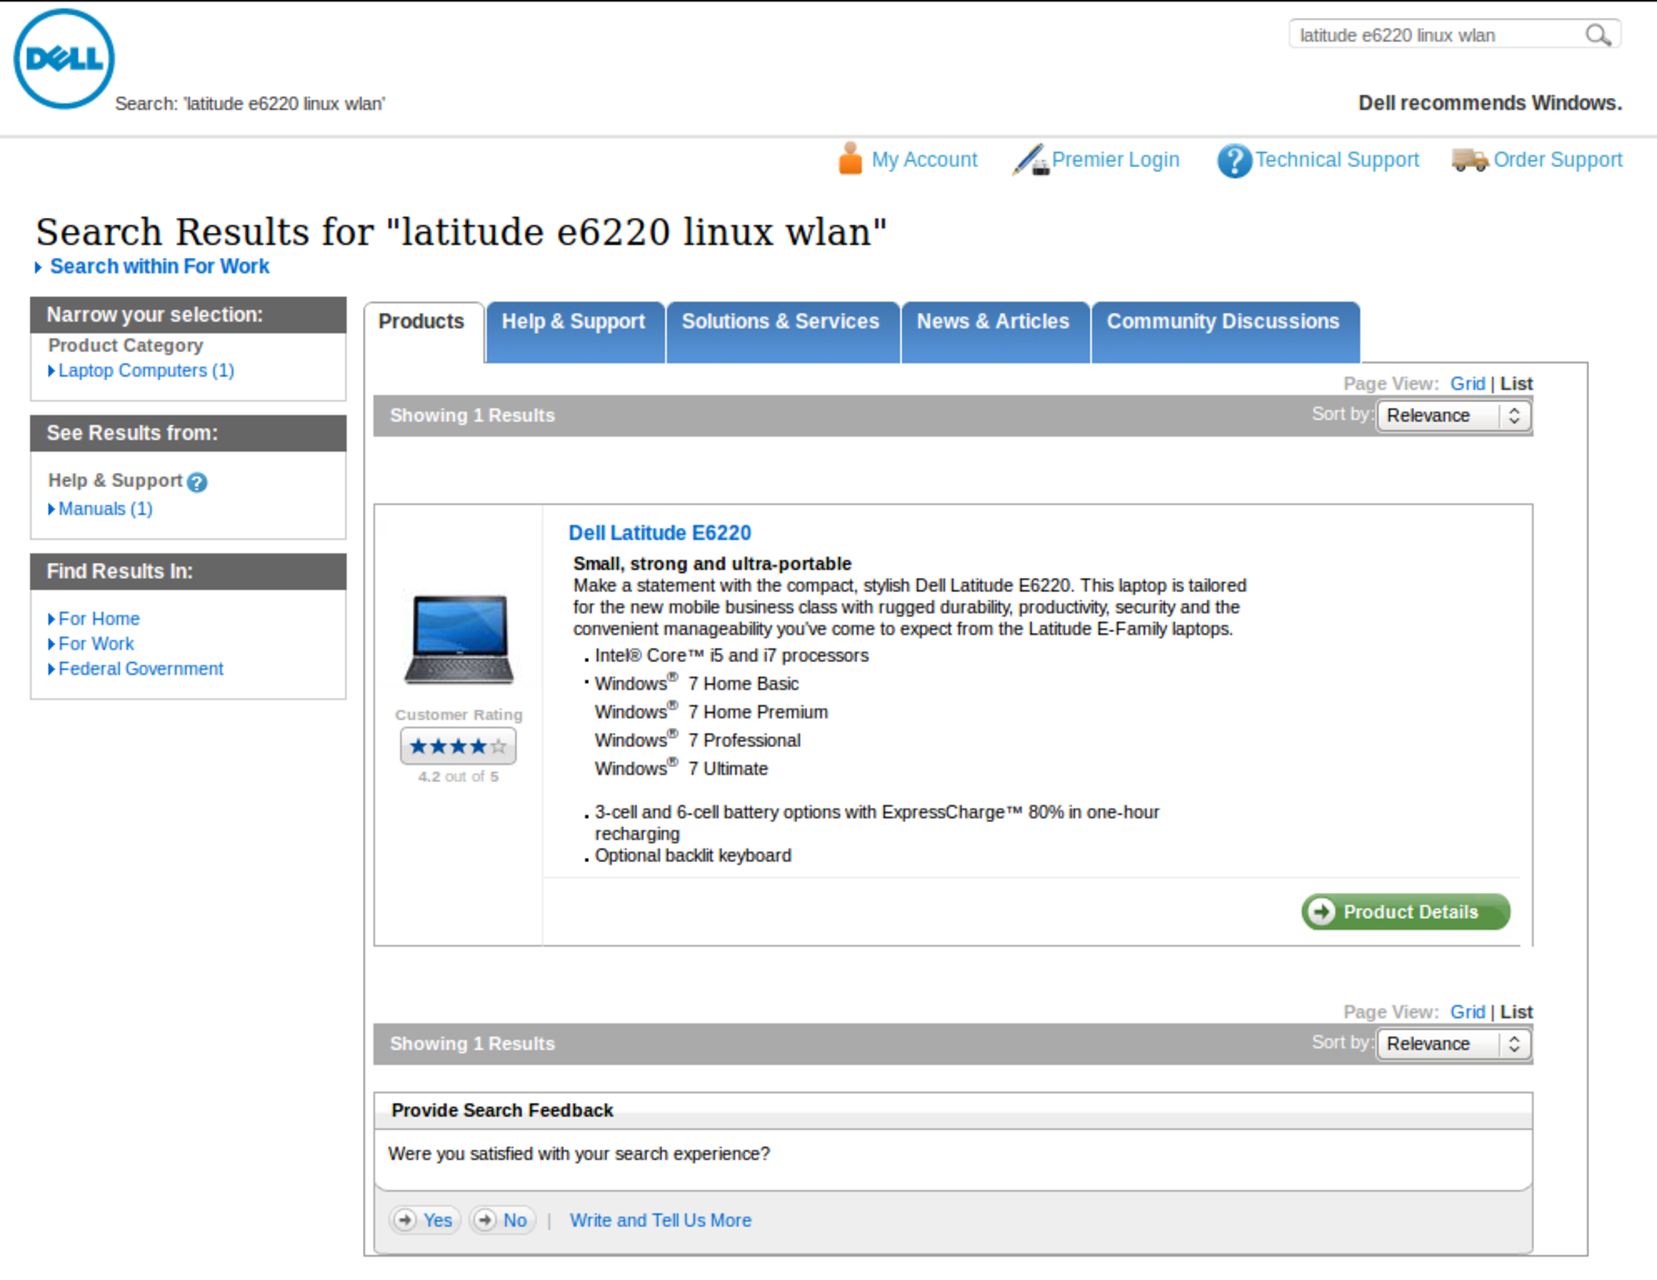
\includegraphics[scale=0.28]{figures/relevanceFeedback1.pdf} 
\end{figure}

\begin{figure}[htp] % t=top, h=here, b=bottom, p=separate page, !=place even if ugly
\caption{Relevance feedback \protect} \label{figure_relevanceFeedback2}
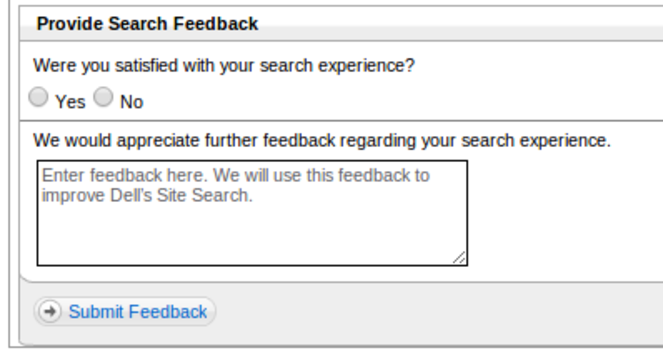
\includegraphics[scale=0.70]{figures/relevanceFeedback2.pdf} 
\end{figure}

\subsection{Query Term Suggestion}

Such search interfaces have appeared that suggest query terms dynamically, as the user enters them.
In some of the systems the term suggestions appear before the searcher has seen any retrieval results, and in others, the system dynamically shows documents that match the characters typed so far, adjusting the results list as more characters are typed.

Dynamic query term suggestions (sometimes referred to as auto-suggest, autosuggest, or search-as-you-type) are becoming a widely used solution between requiring the user to know exactly how to spell the query terms and to think of relevant and connected terms overall. [Hearst]

\begin{figure}[htp] % t=top, h=here, b=bottom, p=separate page, !=place even if ugly
\caption{One view of dynamic query term suggestion. An example from Google in which the prefix of a word in the query is matched against past queries. \protect.} \label{figure_querysuggestion2}
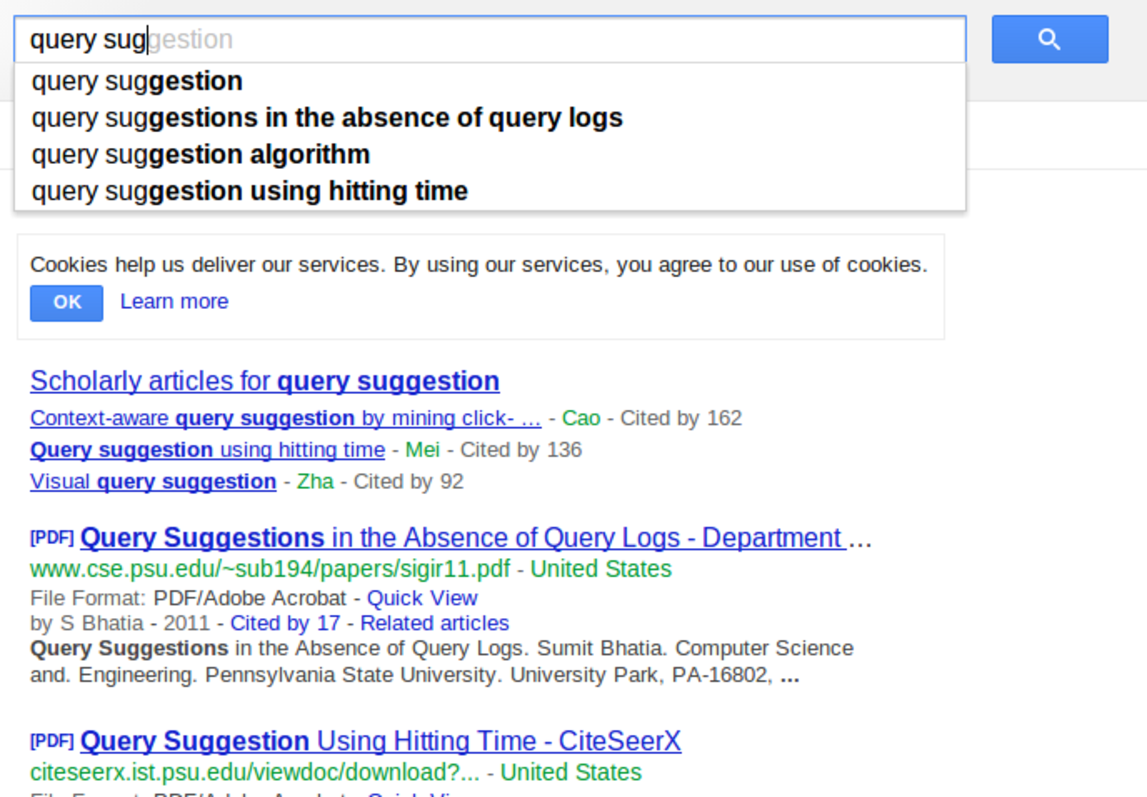
\includegraphics[scale=0.41]{figures/dynamicQueryTermSuggestion2.pdf} 
\end{figure}

Some dynamic term suggestion systems show only query suggestions whose prefix matches what has been typed so far. Figure \ref{figure_querysuggestion2} shows an example from Google's dynamic query suggestions interface, which shows queries where the prefix matches some words used in previously used queries.
In this example, "query sug" matches "query suggestion".
Dynamic query suggestions are not restricted to matching the prefix of the query alone.
In Figure \ref{figure_querysuggestion3} the system detects an upcoming spelling error in user's query term "exansion" and suggests a query with a corrected term "expansion".

\begin{figure}[htp] % t=top, h=here, b=bottom, p=separate page, !=place even if ugly
\caption{Another view of dynamic query term suggestion in Google where the system detects an upcoming spelling error "exansion" and suggests a query including a corrected word, "expansion". \protect} \label{figure_querysuggestion3}
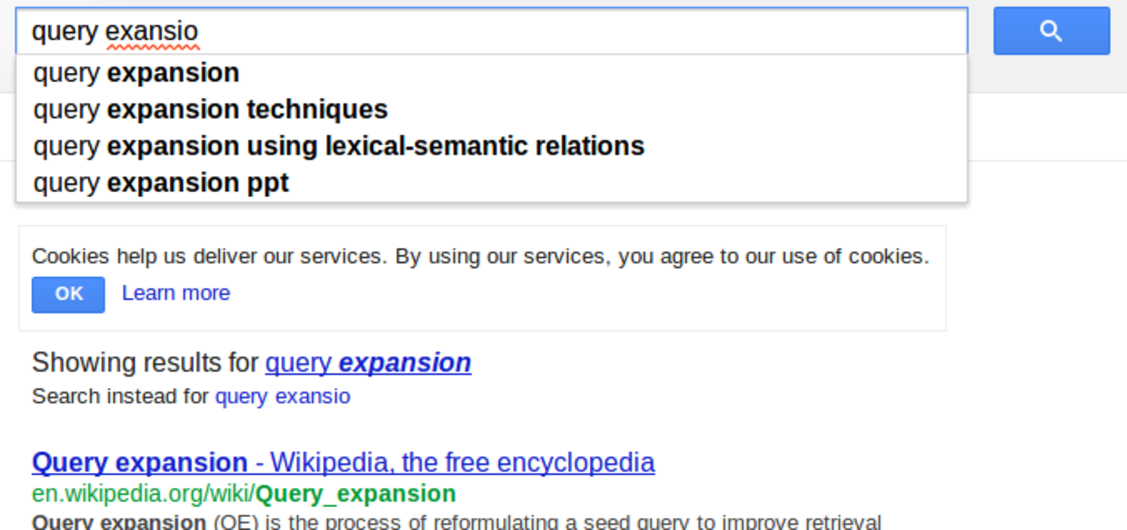
\includegraphics[scale=0.41]{figures/dynamicQueryTermSuggestion3.pdf} 
\end{figure}

A less interactive system is displayed in Figure \ref{figure_queryExpansion3}.
The search system does not suggest any query terms and a user's misspelled query fails.
However, as we see on the right part of the figure, just seconds after the initial use of the word "morgage" the word is used again and spelled exactly the same, but the result page has changed.
This helps user in a similar way as the interactive query suggestion method, but the first use of a word launches a background operation to handle future cases.
The user model of the search system gets updated and after the initial use of the word "morgage" the system will provide a suggestion in the otherwise empty result page.

\begin{figure*}[htp] % t=top, h=here, b=bottom, p=separate page, !=place even if ugly
\caption{Initial use of misspelled query term in Ipswich Borough Counsil website search system results in a page without suggestions (left).
Just seconds following the initial use of misspelled "morgage" query term, we resubmit the query as before and as we see on the right, the system offers "mortgage" as a suggestion.
\protect} \label{figure_queryExpansion3}
\centering
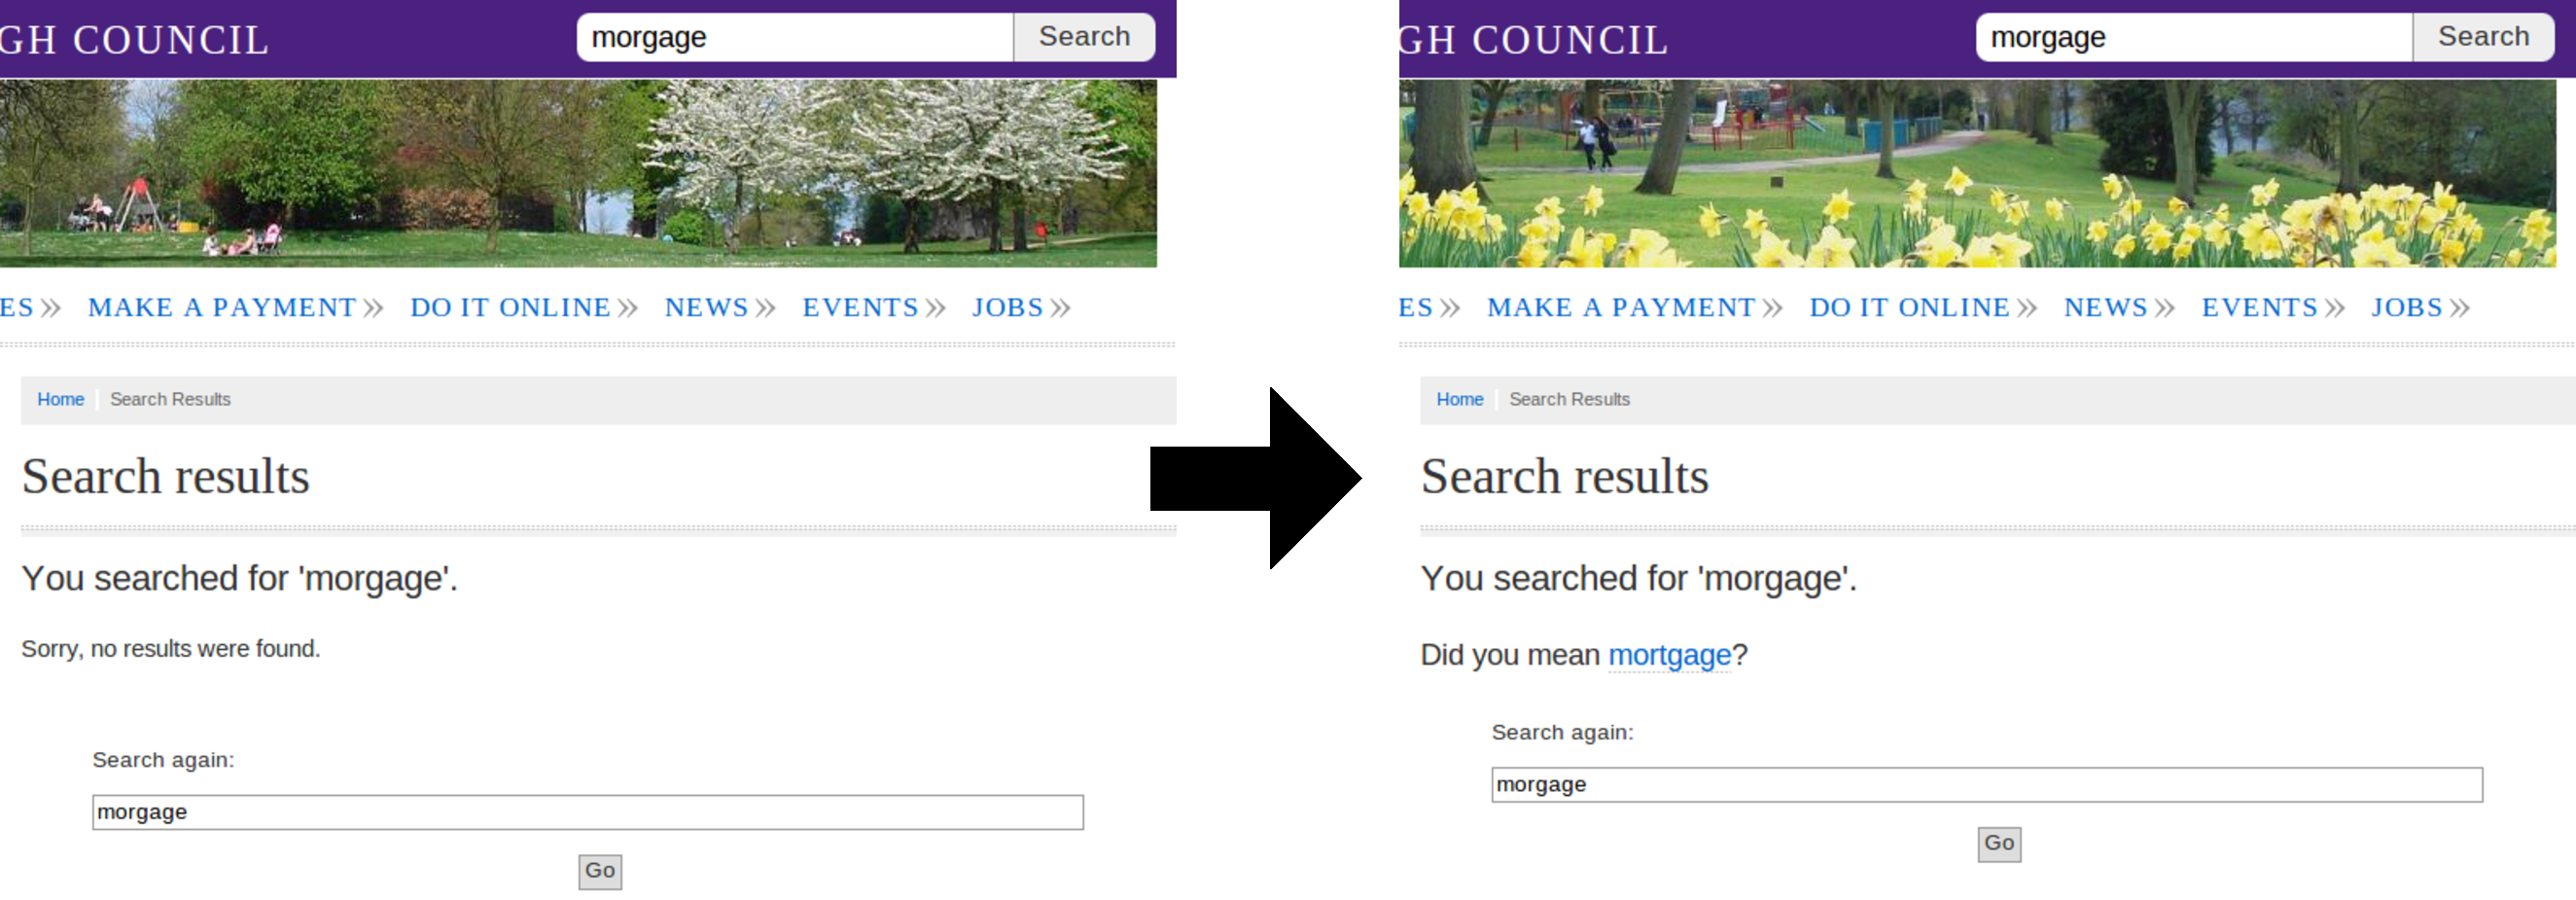
\includegraphics[scale=0.41]{figures/queryExpansion3.pdf} 
\end{figure*}

% include discussion.tex as commands
\section{Discussion}

In the modern day people use online search applications widely. Search applications are actually the second most frequently used online applications. Online environment seems to be perfect for both searching quickly for facts and doing more sophisticated searching with goals like investigating, forming overall understanding of a given subject or trying to learn about previously unknown topics. People's online lives may include anything from finding the perfect companion or watching Psy's next huge viral hit video to learning the basics of physics.  Built on the idea of hyperlinking, the internet is practically made for exploring. Exploratory search tasks have become part of everyday life, maybe because the internet has applications that support it better than the traditional information sources like libraries, books and human-to-human conversations.

Exploratory searchers can be supported in their tasks by means of user modeling, the goal being to accurately model the users' information needs. This task is unfortunately a very difficult one. Indeed, it is hard for users themselves to precisely describe what their information need eventually even is. 

The user interface of an exploratory search system should be designed to fulfill the needs of most of its users. 
More information on what works and doesn't work can usually be collected from system evaluations.
However, evaluating exploratory search systems is difficult, because users have different starting positions.
Their knowledge of the domain varies, they are interested in different aspects of the topic and they have previously encountered different information.
The solutions that aid exploratory search usually include methods to recommend alternative search paths or methods to suggest sources of related information. 

Faceted search has been found to be a useful means of supporting exploratory search. It supports the refining of the query and enables browsing through the formed categories thus enriching the understanding of the knowledge domain. Additionally, the faceted search helps the users to refine or re-evaluate their information needs. Still, even though faceted search interfaces make the search more efficient and the users explore the results more broadly than without facets, they don't always prefer it. 

Another supporting technique that we came upon was query term suggestion.
It saves the user from typing as the system suggests combinations of query terms based on the characters or words the user has already typed in the search form.
A study suggests that as much as 15 percent of search queries return no results because of misspelled query terms.
By clicking a suggested search query, the search gets underway with correctly spelled words and with a certainty that some results will be returned, since the suggested query has successfully been used before.

Most search systems rely only on the query the user has submitted when constructing a user model, but more direct ways to gather information exist, too.
Asking user to rate the result based on its usefulness provides the system with direct and precise evidence of the relevance of the search result.
Relevance feedback has been found effective in enhancing search accuracy, but this method requires a system to analyse given feedback and apply it into the ranking of the search results.
In practise, the extra effort the user needs to make seems to be too much for the users.

In our opinion using user models in supporting exploratory search has some payoffs. The user might feel insecure if the application forms search results for reasons the user does not understand, depriving the user's control of the system. User modeling also has privacy implications. Who stores the information that has been gathered from the user's interactions? How securely it is stored and who controls the purposes it is used for? For example, Google collects information about the user's actions and uses them to construct user model for marketing purposes. The privacy of using the data is questionable and they provide no means of preventing them from collecting one's interaction data. 

The methods we encountered during our literature review were familiar to us as major search engines have incorporated them in their user interfaces, but before writing this paper we didn't know their names, let alone their theoretical background. It is obvious to us that the solutions described in our paper are useful to many exploratory searchers although not all of the implementations we tried were adequately intuitive or mature enough in their visualization.



\section{Conclusions}
Exploratory search is a particularly challenging search task because in many cases even the searchers themselves don't exactly know what they are looking for.
It contains the arduous search activities of learning and investigating and the nature of the task contains a lot of browsing and getting familiar with the concepts of the task domain while it still is uncharted territory.
User modeling in combination with intelligent user interface techniques has the capacity to make exploratory search more efficient and easier for the user.
Faceted search, relevance feedback and query term suggestion are all widely used techniques and they are proven to aid in searching.
User modeling isn't yet to our knowledge combined to faceted search outside research but it has substantial potential as a response for the exploratory search problem.
While exploring the example systems we found two concerning aspects.
Firstly, the feeling of losing control if the system is adapted unpredictably reduces the desire to use the system at all.
Secondly, collecting user data in turn raises a privacy concern; how is user's search data handled and is it used outside the scope of the search system?

\nocite{} %tämä listaa kaikki viitteet luetteloon vaikka niitä ei olisi vielä viitattu

% Balancing columns in a ref list is a bit of a pain because you
% either use a hack like flushend or balance, or manually insert
% a column break.  http://www.tex.ac.uk/cgi-bin/texfaq2html?label=balance
% multicols doesn't work because we're already in two-column mode,
% and flushend isn't awesome, so I choose balance.  See this
% for more info: http://cs.brown.edu/system/software/latex/doc/balance.pdf
%
% Note that in a perfect world balance wants to be in the first
% column of the last page.
%
% If balance doesn't work for you, you can remove that and
% hard-code a column break into the bbl file right before you
% submit:
%
% http://stackoverflow.com/questions/2149854/how-to-manually-equalize-columns-
% in-an-ieee-paper-if-using-bibtex
%
% Or, just remove \balance and give up on balancing the last page.
%
\balance

% If you want to use smaller typesetting for the reference list,
% uncomment the following line:
% \small
\bibliographystyle{acm-sigchi}
\bibliography{umines}
\end{document}
